\documentclass[a4paper]{article}
\usepackage[utf8]{inputenc}
\usepackage{hyphsubst}
%\HyphSubstIfExists{ngerman-x-latest}{
%  \HyphSubstLet{ngerman}{ngerman-x-latest}}{}
%\HyphSubstIfExists{german-x-latest}{
%  \HyphSubstLet{german}{german-x-latest}}{}
\usepackage{zi4}
\usepackage{amsmath} %for matrices
\usepackage{amssymb} %for element of N / R etc
\usepackage{amsthm} % proof
\usepackage[english]{babel} % Beweis etc
\newcounter{theorems}
\usepackage{natbib} % cites
\usepackage{hyperref}

%\usepackage{mdframed}
\usepackage{enumerate}
%\usepackage[hyphenbreaks]{breakurl}

\usepackage{graphicx} %\includegraphics
\usepackage{tikz}
\usetikzlibrary{positioning,fit,patterns}
\usetikzlibrary{shapes}
\usetikzlibrary{arrows}
\usetikzlibrary{arrows.meta}
\usetikzlibrary{positioning,automata} 
\usepackage[all]{xy}
\usepackage{float}
\usepackage{color}
\usepackage{soul} %ul etc
\definecolor{darkgreen}{rgb}{0.0,0.5,0.0}
\definecolor{darkred}{rgb}{0.5,0.0,0.0}
\definecolor{darkyellow}{rgb}{0.5,0.5,0.0}
\definecolor{lightgreen}{rgb}{0.5,1,0.5}
\definecolor{lightgreen2}{rgb}{0.7,0.9,0.7}

\newcommand{\cfbox}[2]{%
    \colorlet{currentcolor}{.}%
    {\color{#1}%
    \fbox{\color{currentcolor}#2}}%
}

\usepackage{listings}
\usepackage{nth}
%\lstset{numbers=left,language=C,frame=lines,commentstyle=\color{darkgreen}\ttfamily,keywordstyle=\color{blue},mathescape,basicstyle=\ttfamily\scriptsize}

\newtheorem{ex}{Example}
\newtheorem*{ex*}{Example}
\newtheorem*{exS}{Example \cite{thwart}}

\newcommand{\matone}{21152466}
\newcommand{\mattwo}{21166929}
\newcommand{\mts}{MTS420cc }
\title{\textbf{Anti Bicycle Theft}\bigskip\\Documentation}
\author{Kevin Freeman (\matone)\\ Martin Schwarzmaier (\mattwo)\\Georg-August-Universität Göttingen}
\date{\today}
\parindent 0pt
\setlength{\parindent}{0pt}

\begin{document}
\setlength\parindent{0pt}
\maketitle
\begin{center}
	\textbf{Practical Course on Wireless Sensor Networks}
\end{center}\vspace{10em}
\begin{center}
	\begin{tabular}{ll}
	\textbf{Lab Advisor: }&Dr. Omar Alfandi\\
	\textbf{Lab Assistants: }&Arne Bochem, M.Sc.
	\end{tabular}
\end{center}

\begin{figure}[b]
	\centering
	
\includegraphics[scale=1]{logo.png} %sehr groß, besser runterskalieren
\end{figure}

\thispagestyle{empty} %Deckblatt, keine Seitenzahl
\newpage

%\renewcommand{\contentsname}{Inhaltsverzeichnis}
\tableofcontents
\thispagestyle{empty} %inhaltsvz, keine Seitenzahl
\newpage

\setcounter{page}{1} %nun Seitennummerierung bei eins beginnen

\section{Introduction}
Bicycle theft is a major concern in many cities. Especially areas that have a high demand for bikes, like university towns, are severely afflicted. In the year 2014 more than 300.000 bikes have been registered as stolen in Germany with many more being stolen but unreported \cite{bka}.\\
Over the last decade many systems have been developed to prevent bicycle theft or to locate stolen bikes. Most of these systems work by using a GPS module for tracking a bike and a GSM module to communicate the data via the mobile phone network \cite{golembike}. Another approach is using a Bluetooth transmitter in combination with a bluetooth and GPS equipped smartphone \cite{leash}. The idea of this approach is to detect if a stolen bike is close to the mobile phone of any user of the system and use the phones positioning capability to log and communicate its approximate position to the owner.\\
In this paper a new approach is proposed. The system envisioned is based on sensor beacons equipped with a GPS module and a close range wireless interface. This wireless interface connects through a system of wireless relay nodes to a base station that is connected to the internet. A user of this system will be able to mark a bike as stolen online. This information will then be disseminated from the base station to all relay stations, possible across several hops. As soon as a bike marked as stolen comes in reach of a relay station it will be informed that is has been stolen. This bike will start to continuously capture GPS coordinates combined with a timestamp and store this information locally. From now on each time the bike comes in reach of a relay station again it will use this station to transmit its stored location data to the base station. From there the tracked positions are made available to the owner via the web interface.\\
This system combines advantages of the existing solutions. By using a GPS module exact locations are obtained making it more exact than using the Bluetooth approach. Also, by storing many locations and dumping them via a short range but high speed wireless connection, a very exact movement history can be created. By providing a relaying infrastructure within a certain area (e.g. a small city) the user is not depending on other users using the system (avoiding a hen-egg problem). At the same time there will be no dependency on mobile network providers and therefore fees imposed by them.\\

\section{Environment}
Before presenting the project we firstly show what the whole environment looks like. Firstly, IRIS motes\footnote{A full description can be found at \url{http://www.memsic.com/userfiles/files/Datasheets/WSN/IRIS_Datasheet.pdf}} are used (see Figure \ref{fig:mote}). Programs for the motes are written in nesC\footnote{\url{http://www.tinyos.net/api/nesc/doc/ref.pdf}}, compiled and flashed with tinyOS. Additionally, the computer used provides packages mentioned in Section \ref{sec:walkthrough} and is connected to a base station via USB Gateway, which can be seen in Figure \ref{fig:gateway}. Some of the motes are connected to a \mts sensorboard (see Figure \ref{fig:420cc}). A GPS antenna is attached to the sensorboards.\footnote{Figure \ref{fig:mote}, \ref{fig:gateway} and \ref{fig:420cc} have been take from \url{https://user.informatik.uni-goettingen.de/~sensorlab/Hardware.php}}
\begin{figure}[h!]
\begin{center}
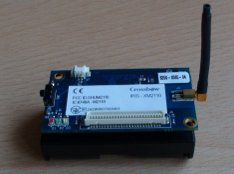
\includegraphics[scale=0.75]{pics/mote.jpg}
\caption{Standard IRIS mote without sensorboard.}
\label{fig:mote}
\end{center}
\end{figure}
\begin{figure}[h!]

\begin{center}
\begin{minipage}{0.47\textwidth}
\begin{center}
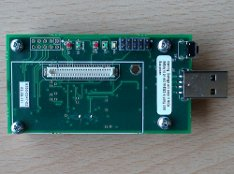
\includegraphics[scale=0.5]{pics/gateway.jpg}
\caption{USB Gateway, used to forward packets via USB.}
\label{fig:gateway}
\end{center}
\end{minipage}
\begin{minipage}{0.06\textwidth}
\end{minipage}
\begin{minipage}{0.47\textwidth}
\begin{center}
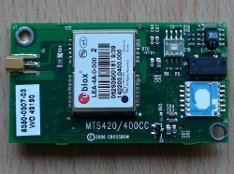
\includegraphics[scale=0.5]{pics/420cc.jpg}
\caption{\mts sensorboard, able to process GPS signals.}
\label{fig:420cc}
\end{center}
\end{minipage}

\end{center}

\end{figure}

Our test environment used the following Linux packages:
\begin{enumerate}
\item nodejs (version 5.5.0)
\item python2 (version 2.7.11)
\item mongodb (version 3.2.0)
\item jdk7-openjdk (version 7.u95\_2.6.4)
\item python2-pymongo (version 3.2)

\end{enumerate}

\section{Walkthrough}\label{sec:walkthrough}
This section demonstrates the project without showing technical details, as they will be explained in Section \ref{sec:insight}. 
\subsection{Flashing the motes}
In order to make this project work, at least one IRIS mote is needed as a base station as well as at least one iris mote equipped with a \mts board including a GPS antenna. Each additional bicycle will need an identical sensorboard and GPS antenna. Additionally, it is possible to extend the network range with extra motes. This brings us to the following summary of needed motes:
\begin{enumerate}
\item[a)] one base station \texttt{[./nesC/base\_station]}
\item[b)] one \mts sensorboard with GPS antenna per bicycle \texttt{[./nesC/bike]}
\item[c)] any amount of network node motes \texttt{[./nesC/nodes]}
\end{enumerate}
\subsection{Starting MongoDB, NodeJS and SerialForwarder}
As the whole project is supposed to be user friendly, a webserver (Node.js) is implemented attached to a database (MongoDB).
The webserver can be started by running the following command and will be available under \texttt{localhost:8080} afterwards:
\begin{lstlisting}[frame=single,language=bash]
$ node ./webapp/app.js
\end{lstlisting}
Additionally, the MongoDB daemon has to be started:
\begin{lstlisting}[frame=single,language=bash]
# mongod
\end{lstlisting}
Now the user is able to register to the webservice and mark his or her bicycles as stolen as shown in Figure \ref{fig:webregistration} and \ref{fig:mark}. Once GPS data is collected, the user is able to view it on using the same webapp, as seen in Figure \ref{fig:GPSdata}.
\begin{figure}[h!]
\begin{center}
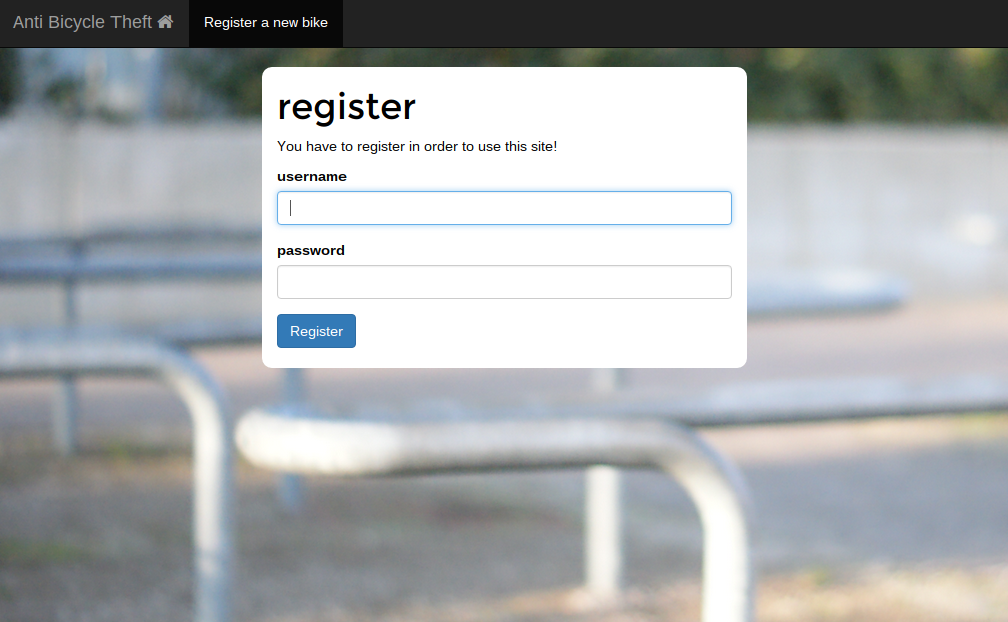
\includegraphics[keepaspectratio=false, width=12cm, height=8cm]{pics/reg.png}
\end{center}
\caption{Registration website}
\label{fig:webregistration}
\end{figure}
\begin{figure}
\begin{center}
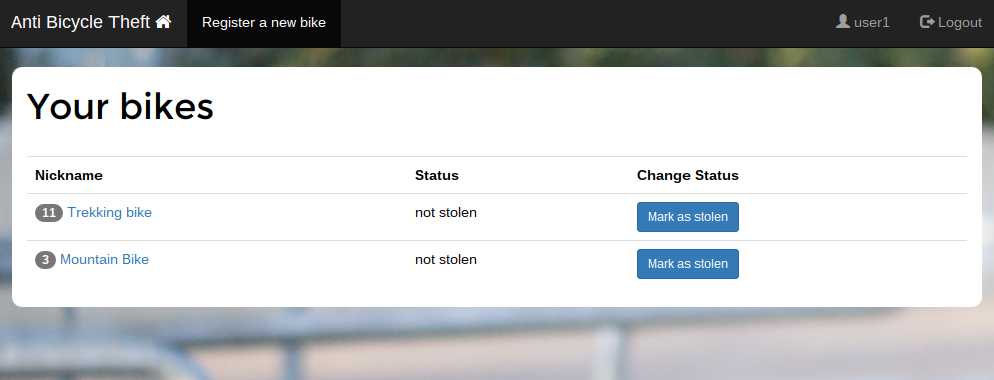
\includegraphics[keepaspectratio=false, width=12cm, height=5cm]{pics/mark.png}
\end{center}
\caption{Viewing registered bikes}
\label{fig:mark}
\end{figure}
\begin{figure}
\begin{center}
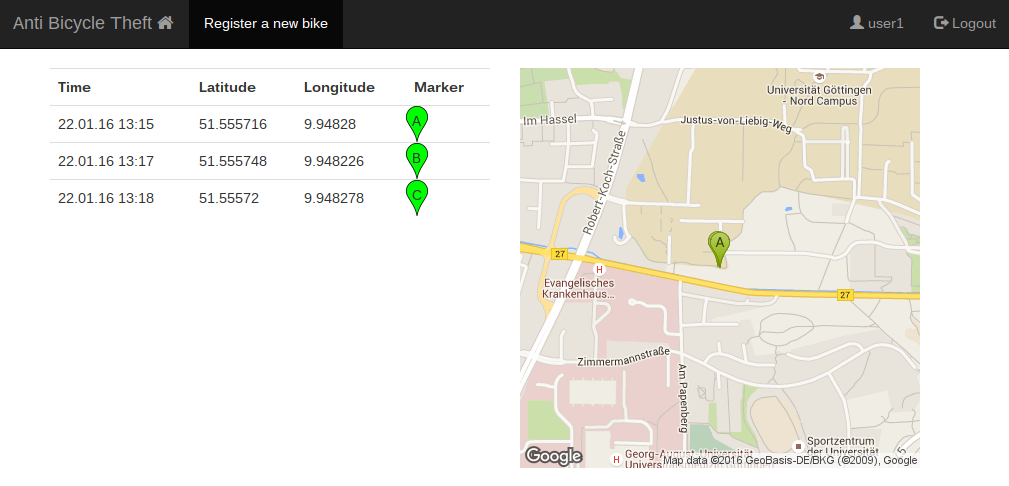
\includegraphics[keepaspectratio=false, width=12cm, height=6cm]{pics/view.png}
\end{center}
\caption{Viewing gathered GPS coordinates}
\label{fig:GPSdata}
\end{figure}

Another connection to the database is established by the base station via python, which is calling the java classes \texttt{\path{net.tinyos.tools.Send}} and \texttt{\path{net.tinyos.tools.Listen}}. These are available after starting the \texttt{SerialForwarder} with:
\begin{lstlisting}[frame=single,language=bash]
$ java net.tinyos.sf.SerialForwader
                            -comm serial@/dev/ttyUSB1:iris
\end{lstlisting}
Afterwards, only the \texttt{listen.py} has to be run, which imports our \texttt{\path{./python-api/env/bikeDB/bikeDB.py}} script. This will enable automatic gathering of stolen bicycle \texttt{ID}s from the database and push them into the network, but will also collect GPS coordinates from bicycles and save them in the database.
\begin{lstlisting}[frame=single]
$ python2 ./python-api/env/bikeDB/listen.py
\end{lstlisting}

\section{Network Protocols and Mote Insight}\label{sec:insight}%TODO: clever sectionname here
As the walkthrough only showed how to use the project, this section shows programs and protocols used for each mote in detail. As all motes are supposed to talk with each other, one superior header file is implemented. It provides easy changeable variables for the maximal amount of bicycles, that can be marked as stolen at the same time as well as how many GPS coordinates are transmitted in a single packet as seen in Listing \ref{lst:datamsg}. The gathering process uses the Collection protocol \cite{colldiss}. Contrary, the propagation of stolen bicycle \texttt{ID}s is done via the Dissemination protocol \cite{colldiss}. 
\begin{lstlisting}[numbers=left, frame=single,language=C, captionpos=b, caption={DataMsg.h, content of packets}, label=lst:datamsg]
//...
#define MAXBIKES 10
#define COORDS_PER_PACKET 2
typedef nx_struct EasyDisseminationMsg 
{
    nx_uint16_t bikes[MAXBIKES];
} EasyDisseminationMsg;
//...
typedef nx_struct EasyCollectionMsg 
{
    nx_uint16_t nodeid;
    nx_uint32_t current_time;
    nx_uint32_t time[COORDS_PER_PACKET];
    nx_uint32_t lat[COORDS_PER_PACKET];
    nx_uint32_t lon[COORDS_PER_PACKET];
} EasyCollectionMsg;
\end{lstlisting}
Obviously, the content and variable types can be changed easily, too.
\subsection{Base Station}
Our base station \texttt{[./nesC/base\_station]} is connected to a computer via USB. On this computer, a \texttt{SerialForwarder} is run in order to establish a possibility to send and receive data to and from the base station. For this project, on the one hand, we have to push \texttt{ID}s of stolen bikes to the base station in order to disseminate them through the network. On the other hand, the collection protocol is used to gather information from stolen bikes, like coordinates. This is done via a python script, which can be seen in Listing \ref{lst:listen.py}. In line 3 it imports our bikeDB class, which is simply providing methods to read and write to the database.\\

\subsection{Network Node}
The network nodes are completely omittable as they only enlarge the network. More network nodes are needed if the availability of the network needs to be increased. These are connected with other network nodes and disseminate and collect the data mentioned already to and from the base station and bicycle motes. Currently, they are doing nothing but disseminating and collecting. However, functionality can be easily added in the \texttt{\path{./nesC/nodes/NodeC.nc}}.
\subsection{Bicycle Mote}
Bicycle motes are attached to each bicycle and equipped with a \mts sensorboard including GPS antenna.\\
Each of them has a unique identifier (\texttt{ID}), which is used to link a mote to a bicycle. Through the webapp the user is then able to mark his bicycle as stolen. Afterwards, the \texttt{ID} is disseminated through the whole network. If the bicycle approaches a network node, it receives a dissemination packet. These are called "pings". As the bicycle now knows that the network is in range and available, it will check, if its own \texttt{ID} is marked as stolen. If so, the GPS antenna is powered on and starts approximately 90 seconds later to save data (current runtime, latitude, longitude).\\
After recording data successfully and receiving another ping, the bicycle mote will dump the data into the network using the collection protocol.\\

Each mote has a RAM of 8 kB. Therefore, it is possible to store 600 coordinate-tuples on the bicycle mote RAM. As we are approximately storing one tuple every 3 minutes, it is possible to store the coordinates of the last 30h. This can be extended by saving onto the measurement flash itself, which we left out for future work, as 30h is enough for all our testcases and the battery time is limited due to usage of GPS as well.

\subsection{Topology}
Figure \ref{fig:topo} shows an example topology with one base station, four network nodes and one bicycle mote that is in range of the network. Therefore, it will be able to receive the stolen bicycle \texttt{ID}s and check, if it is marked as stolen.
\begin{figure}[h!]
\begin{center}
\begin{tikzpicture}[node distance=1.5cm]

%CLOUD
\node [cloud, draw,cloud puffs=10,cloud puff arc=120, aspect=2, inner ysep=1em](cl) at (-0.3,4) {Internet};

\node[ellipse, draw, thick, fill=blue!20](bs) at (-1,2){Base Station};

\node[circle, draw, thick, fill=blue!20](n1) at (0,0){Node$_1$} ;
\node[circle, draw, thick, fill=blue!20, right = of n1](n2){Node$_2$};
\node[strike out, draw,rotate=-50,ultra thick, fill=blue!20] at (2,-1.5){obstacle};
\node[circle, draw, thick, fill=blue!20](n3) at (1,-3){Node$_3$};
\node[circle, draw, thick, fill=blue!20](n4) at (4,-3.5){Node$_4$};

\node[rotate=0](bike) at (-1,-4){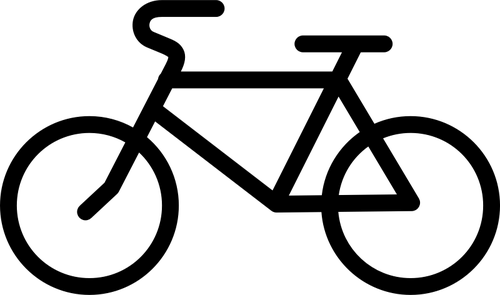
\includegraphics[width=.1\textwidth]{bicycle.png}};

\draw[->, arrows={Triangle-Triangle}] (bs) -- (cl);
\node at (-0.4,2.75){PC} ;

\draw[->, arrows={-Triangle}, draw=red, transform canvas={xshift = 0.05cm}] (bs) -- (n1);
\draw[->, arrows={-Triangle}, draw=green, transform canvas={xshift = -0.05cm}] (n1) -- (bs);

\draw[->, arrows={-Triangle}, draw=red, transform canvas={xshift = 0.05cm}] (n1) -- (n3);
\draw[->, arrows={-Triangle}, draw=green, transform canvas={xshift = -0.05cm}] (n3) -- (n1);

\draw[->, arrows={-Triangle}, draw=red, transform canvas={yshift = 0.05cm}] (n1) -- (n2);
\draw[->, arrows={-Triangle}, draw=green, transform canvas={yshift = -0.05cm}] (n2) -- (n1);

\draw[->, arrows={-Triangle}, draw=red, transform canvas={xshift = 0.05cm}] (n2) -- (n4);
\draw[->, arrows={-Triangle}, draw=green, transform canvas={xshift = -0.05cm}] (n4) -- (n2);

\draw[->, arrows={-Triangle}, draw=red, transform canvas={yshift = 0.05cm}] (n3) -- (n4);
\draw[->, arrows={-Triangle}, draw=green, transform canvas={yshift = -0.05cm}] (n4) -- (n3);

\draw[->, arrows={Triangle-}, draw=red, transform canvas={yshift = 0.05cm}] (n3) -- (-0.5,-3.75);
\draw[->, arrows={Triangle-}, draw=green, transform canvas={yshift = -0.05cm}] (-0.5,-3.75) -- (n3);

\filldraw[color=green] (3-1,2+0.5) rectangle (3.5-1,2.5+0.5);
\node at (4.375-1,2.25+0.5)  {Collection};
\filldraw[color=red] (3-1,1.5+0.5) rectangle (3.5-1,2.0+0.5);
\node at (4.7-1,1.75+0.5)  {Dissemination};
\filldraw[color=black] (3-1,1.0+0.5) rectangle (3.5-1,1.5+0.5);
\node at (4.85-1,1.25+0.5)  {SerialForwarder};




\end{tikzpicture}
\end{center}
\caption{Example network including protocols used}\label{fig:topo}
\end{figure}

\section{Evaluation and Conclusion}
The project was tested several times by flashing the programs onto different motes. All components are working as described. Motes were marked as stolen via the website. The stolen \texttt{ID}s were disseminated without problems. Afterwards, corresponding bicycle motes started to record data. Even when a bicycle mote left the network for some time, the recorded data was collected successfully after entering the network again. This data is correctly shown on the webapp as shown in Figure \ref{fig:concl}. However, the GPS antenna may lose the signal and therefore returns faulty coordinates. These are omitted upon collection at the base station (line 64 of Listing \ref{lst:listen.py}).
All in all the project approach is working very well and is able to run long enough to gain necessary information, e.g. where the bicycle is placed at night (this might be the home of the thief). The main disadvantage is the great power consumption by the GPS module. To eliminate this disadvantage, it should be possible to charge the battery while cycling or, for example, use solar energy. Furthermore, the GPS antenna could be powered off if the same coordinates are received for a certain period of time. These aspects are presented in the next section.

\begin{figure}[h!]
\begin{center}
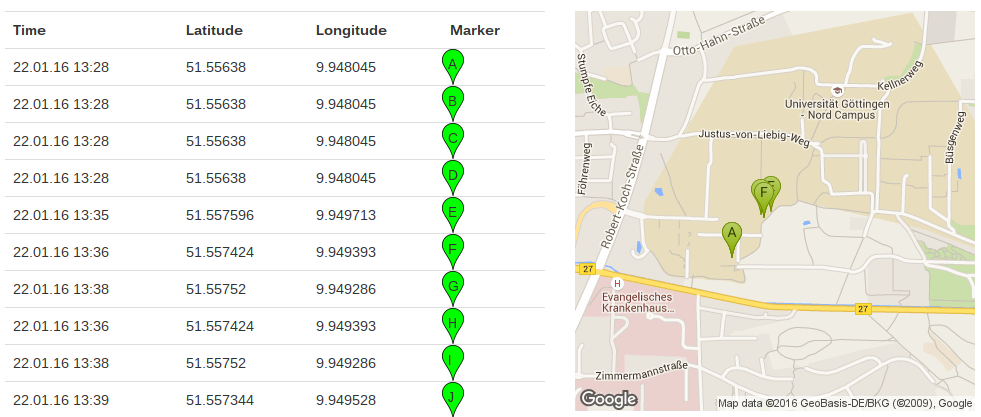
\includegraphics[scale=0.35]{pics/concl.png}
\caption{Captured packets after walking outside.}
\label{fig:concl}
\end{center}
\end{figure}

\section{Future Aspects}
The projects objective is to point out the possibility of a new tracking system using IRIS motes. Therefore, some additions have been left out, as they would not change the procedure, but increase the security, for example. All of these points are explained in this section.
\begin{enumerate}
\item \textbf{Privacy and authentication}. Obviously, administrators of the webapp are able to access data of users and mark specific bicycles as stolen, to start the gathering process. Therefore, the GPS data gathered could be encrypted using asymmetric cryptography. The user will receive encrypted data and decrypt it using a private key.
\item \textbf{Encrypted traffic}. Relating to the previous point, the whole traffic of the network, including dissemination of stolen bicycle \texttt{ID}s, should be encrypted to ensure privacy and integrity of packets.
\item \textbf{Further dissemination of stolen IDs}. Bicycle motes, regardless of their state, could save and disseminate the \texttt{ID}s of stolen bicycles. This way, a bicycle would be able to start gathering data without connecting to the relay network, but to another bicycle. Obviously, one has to take care of synchronicity in this case.
\item \textbf{Measurement flash}. Instead of just keeping the gathered GPS data in the memory, one could save them to the flash of the mote and load them again when receiving a ping of the network. This provides the possibility to store a huge amount of coordinates.
\item \textbf{Battery life}. When implementing the previous mentioned point, the battery life has to be extended as well as GPS needs a lot of battery. However, one could use two approaches:
\begin{enumerate}
\item A stolen bicycle is going to be used. Therefore, one could power the mote using the energy of a dynamo attached to the bicycle.
\item At some places, for example a basement, the GPS antenna is not able to maintain a connection. Hence, the GPS antenna could be powered off after e.g. 1 minute without connection. Afterwards, the GPS module is started again after a small amount of time and checks for connection again.
\end{enumerate}
\item \textbf{Hiding of the mote}. The thief should not see and be able to remove the mote from the bicycle. So the mote has to be hidden somewhere in the frame of the bicycle without losing signal.
\item \textbf{GPS exchangeability}. As GPS drains a lot of battery, one could think of implementing a wifi scanner instead of GPS. As wifi is widely used, wifi networks can be found almost everywhere. Using the \texttt{SSID}s only (without connecting to them) the current location can be determined within a certain range. This obviously consumes less power than GPS and will even work, if a bicycle is e.g. in a garage, where a GPS antenna will not be able to establish a connection.
\end{enumerate}


\section{Appendix - relevant code passages}
\subsection{./nesC/base\_station}
Receiving stolen bicycle IDs from PC
\begin{lstlisting}[numbers=left, frame=single,language=C, captionpos=b, caption={BaseStationC, reading out stolen bike \texttt{ID}s}, label=lst:xxx,firstnumber=292]
//...
for (i=0;i<MAXBIKES;i++)
{
    pkt.bikes[i]=msg->data[i*2]*256+msg->data[i*2+1];
}
//...
\end{lstlisting}

\subsection{base\_station}
Receiving stolen bicycle IDs from PC
\begin{lstlisting}[breaklines=true, numbers=left, frame=single,language=C, captionpos=b, caption={DataMsg.h, content of packets}, label=lst:xxx]
#define MAXPOSITIONS 100
//...
uint32_t lons[MAXPOSITIONS];
uint32_t lats[MAXPOSITIONS];
uint32_t times[MAXPOSITIONS];

//reading coordinates in RAM
atomic
{
    for (i=current_reading_pos;i!=current_writing_pos;i++)
    {
        msg->time[j] = times[i];
        msg->lat[j] = lats[i];
        msg->lon[j] = lons[i];
        times[i]=0;
        lats[i]=0;
        lons[i]=0;
        current_reading_pos++; //we read the value
        if (current_reading_pos==MAXPOSITIONS)
            current_reading_pos=0;

        j++;
        if (j==COORDS_PER_PACKET)
            break;
    }    
}

//writing coordinates to RAM
atomic
{
    lats[current_writing_pos]=(uint32_t)(lat*1000000);
    lons[current_writing_pos]=(uint32_t)(lon*1000000);
    times[current_writing_pos]=(uint32_t)((call LocalTimeMicro.get())/1000); //3digits ms
    current_writing_pos++;
    if (current_writing_pos==MAXPOSITIONS)
        current_writing_pos=0;
    call Leds.led0Toggle();
}   

//receiving IDs and starting GPS if stolen
event void Value.changed() 
{
uint8_t i;
const EasyDisseminationMsg* newVal = call Value.get();
bool found=FALSE;
pkt = *newVal;
for (i=0;i<MAXBIKES;i++)
{
    if (pkt.bikes[i]==secret())
    {  
        stolen=0x01;
        found=TRUE;
        call Leds.led1On();
        if (gps_started==0)
        {
            gps_started=1;
            call Timer.startOneShot(90000); //wait X/1000 secs
            call GpsControl.start();
        }
        else if (gps_started==2) //startDone for GPS
        {   
            call Leds.led2Toggle();
            //it is stolen AND received a broadcast 
            //=> DUMP ONE PACKET
            sendMessage(); 
        }
    }
}
if (found==FALSE)
{
    call Leds.led1Off();
    stolen=0x00;
    if (gps_started>1)
    {
        call GpsControl.stop();
        gps_started=0;
    }
}
\end{lstlisting}

\begin{lstlisting}[breaklines=true, numbers=left, frame=single,language=python, captionpos=b, caption={listen.py, receiving and sending via python2}, label=lst:listen.py]
import subprocess
import time
import bikeDB
import datetime
import thread
import os

maxBikes=10

def unsecret(secret):
    return (secret-9)/7

def send(bDB):
    while True:
        stolen=bDB.getIdsOfStolen()
        cmd="java net.tinyos.tools.Send "
        pkt="00 FF FF 00 04 %02x FE 2A "
        packetlength=2
        stolen_str=""
        for b in stolen:
            stolen_str+="%02x %02x "%(int(b)/256,int(b)%256)
            packetlength+=2
        for i in range(maxBikes-len(stolen)):
            stolen_str+="00 00 "
            packetlength+=2
        if packetlength>2: 
            pkt = pkt % packetlength
            pkt = pkt + stolen_str
            cmd = cmd + pkt.upper()
            print("send: {}".format(pkt))
            print(cmd)
            os.system(cmd)

        time.sleep(3);


def recv(bDB):
    #p = subprocess.Popen(["java net.tinyos.tools.Listen -comm serial@/dev/ttyUSB1:iris &"], stdout=subprocess.PIPE, shell=True)
    p = subprocess.Popen(["java net.tinyos.tools.Listen &"], stdout=subprocess.PIPE, shell=True)  # use this WITH serialForwarder
    COORDS_PER_PACKET=2
    LENGTH_OF_PACKET=(2+4+4+4)*2 #in nibbles
    while True:
        pkt=p.stdout.readline().strip(" \n\r\t").lower()  #reads until \n
        pkt=pkt.replace(" ","")
        print("recv: {}".format(pkt))
        if (pkt[30:32]=="ee"): #dissemination ID
            nodeid=pkt[32:36]
            print "sent by:",unsecret(int(nodeid,16)),"(%s)"%nodeid
            runtime=int(pkt[36:44],16)/1000.0
            print "runtime:",runtime
            offset=44
            for i in range(0,COORDS_PER_PACKET):
                t=int(pkt[offset+i*8:offset+i*8+8],16)/1000.0
                lat=int(pkt[offset+i*8+COORDS_PER_PACKET*8:offset+i*8+COORDS_PER_PACKET*8+8],16)/1000000.0
                lon=int(pkt[offset+i*8+COORDS_PER_PACKET*8+COORDS_PER_PACKET*8:offset+i*8+COORDS_PER_PACKET*8+COORDS_PER_PACKET*8+8],16)/1000000.0
                
                print "time:",t
                print "lat:",lat
                print "lon:",lon
                timestamp=datetime.datetime.fromtimestamp(time.time()-int(runtime-t)).isoformat()
                print "timestamp:",timestamp
                print "insert:","%d"%int(nodeid,16),
                print lat,lon,timestamp
                if (lat<99 and lon<99 and lat!=0.0 and lon!=0.0):
                    bDB.insertPosition("%d"%int(nodeid,16),str(lat),str(lon),timestamp)
                #lat = pkt[


if __name__ == "__main__":
    bDB = bikeDB.BikeDB()
    thread.start_new_thread(send,(bDB,))
    recv(bDB) # blocking
\end{lstlisting}


%\newpage
\section{References}\vspace{-2.5em}
\renewcommand\refname{}
%\nocite{pgraph}
%\nocite{clrs2}
%\nocite{wiki}
\bibliographystyle{plain}
\bibliography{src}{}

%
\end{document}
